\section{Multicore}
Performance steigerung durch Clockfreq. erhöhung (erhöht jedoch Verlustleistung linear - Hitzeprolematik) oder Instruktions-Level parallelism (zB DSP) oder Thread-level. Bei Thread-Level gibt es die möglichkeit, Uniprocessor durch time-slicing oder mit Mulitprozessoren  echte TLP zu erreichen. Dafür muss der Speicher korrekt organisiert werden.

\begin{center}
	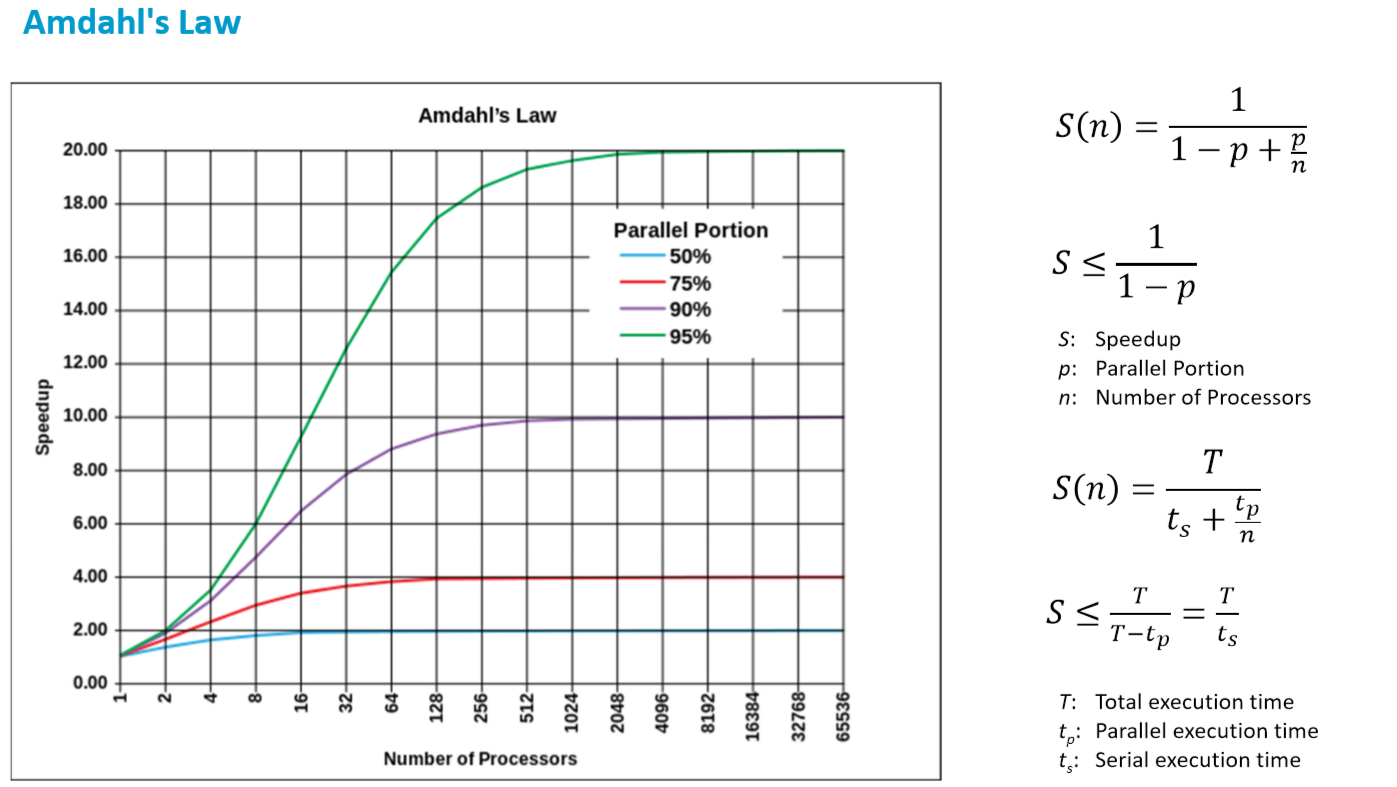
\includegraphics[width=\columnwidth]{Images/amdahls}
\end{center}

\subsection{Caches}
Caches führen eine Kopie von häufig benötigten Speicherdaten aus. Im besten Fall sind Daten bereits im Cache vorhanden (Cache Hit). Dann ist es viel schneller als wenn die CPU Daten aus dem Hauptspeicher laden muss (Cache Miss). 
\begin{center}
	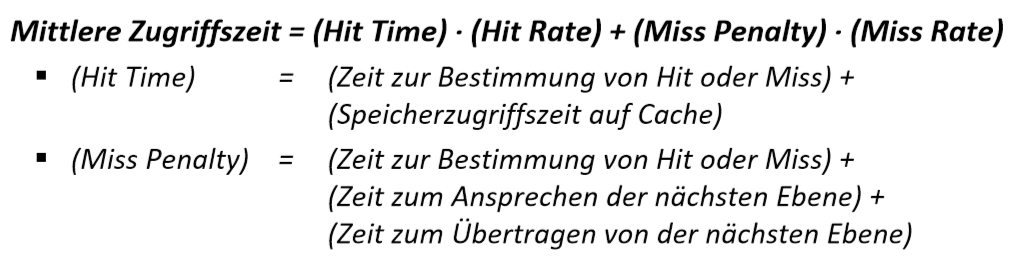
\includegraphics[width=\columnwidth]{Images/mittlerewartezeit}
\end{center}

Als Alternative zur mittleren Wartezeit ist die Worst Case Execution Time (WCET) definiert. Die WCET ist mit einem Cache schlechter, da zum eigentlichen Zugriff immernoch die Bestimmung ob Hit oder Miss hinnzukommt. Ein Cache senkt nur die \textbf{mittlere} Wartezeit! Daher sind caches in in vielen harten Echtzeitsystem nicht erwünscht.

Um beim laden einer Variable zu verhindern, dass dieser im Cache liegt, muss diese mit dem Keyword volatile definiert sein. Dies bewirkt, dass eine CPU die Variable immer frisch aus dem Hauptspeicher liest, und nicht eine Kopie verwendet, was bei Multicore system zu fehlern führen kann.